%!TEX root = thesis.tex
\chapter{Interconnect}
\label{sec:interconnect}
ReconOS provides exceptional transparency regarding the implementation and
execution mode of a thread over the hardware/software boundary. However, the
delegate mechanism introduces an overhead for communication between threads
running in hardware. While for computational intensive tasks with low
communication demand the overhead is acceptable, for low-latency applications
with real-time aspects it breaks the overall performance significantly.
Especially for \acp{PAC}, utilizing the \ac{FPGA} for low-latency and
performance critical parts of the controller, a fast communication is crucial.

This chapter addresses the topic of communication overhead and investigates
ways to speedup the on-chip communication without loosing transparency or
burden the developer with additional tasks. Starting with a short description
of the current system, different approaches from the literature are discussed
and compared. The final architecture is then presented and evaluated.

\section{Limitations of Delegate Mechanism}
While the basic concepts of the delegate mechanism were already discussed in
the background section, a detailed knowledge of its implementation and
performance limitations is required. Consider figure \ref{fig:delegate},
showing a detailed view of the delegate implementation, consisting out of
communication interfaces, interrupt lines and drivers.
\begin{figure}
	\centering
	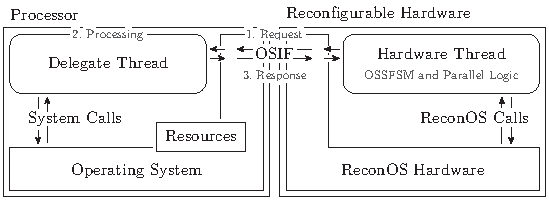
\includegraphics[width=12cm]{../figures/delegate}
	\caption{ReconOS delegate mechanism in detail}
	\label{fig:delegate}
\end{figure}
 The \ac{OSIF} connects the hardware slot with the delegate thread as a
bidirectional \ac{FIFO} interface and allows message based communication. The
\acp{FIFO} are implemented in the reconfigurable fabric and attached to the
\ac{AXI} bus via an interface bridge. It provides access from the \ac{CPU} by
a set of memory mapped register and allows to read status bits or data words.
Furthermore, the \ac{OSIF} is attached to the interrupt input of the processor
to avoid busy waiting in the delegate threads. They are waiting for requests
from the hardware threads and consume no processing time on the processor
while being blocked in a system call. The driver module provides access to the
\ac{OSIF} via a message based protocol accessing the memory mapped register
and handling interrupts.

To illustrate the procedure of delegating an \ac{OS} call, figure
\ref{fig:delegate} sketches an exemplary \lstinline{MBOX_GET}. At first, the
hardware thread issues the request by writing messages into the \ac{OSIF},
namely an internal encoding of the command followed by an identification of
the appropriate \ac{OS} resource and additional arguments. The interrupt
causes the delegate thread to wake up, read the messages from the \ac{OSIF}
and decode the commands. After executing the appropriate \ac{OS} call, the
delegate thread writes back an acknowledge into the \ac{OSIF} and, optionally,
the result of the system call. Following this process, the exchange of a
single message between two hardware threads via a mailbox includes two
interrupts implying context switches into the kernel space, the handling of
the mailbox by the kernel and the access of the \ac{OSIF}. All these
operations introduce a significantly delay of thousands of clock cycles and
burden the processor with additional tasks. Furthermore, since the benefits of
a custom hardware implementation originate from its highly parallel
structures, the sequential execution enforced by the communication via the
central processor results in a bottleneck, limiting the full potential of all
hardware threads.

Besides the communication via system calls and synchronization primitives
handled by the delegate mechanism, the threads are also allowed to exchange
data via the shared memory interface. It provides access to the main memory
but introduces the same bottleneck of enforcing access in a sequential manner.
Again, the benefits of parallel execution are narrowed and performance is
decreased. In particular, streaming-like applications passing data from one
thread to the other cannot be modeled efficiently by applying a shared memory
model. Instead, a method of exchanging data directly from one thread to the
other is required.

\section{Interconnect Architecture}

Introducing a method of communication for hardware threads without involving
the processor includes several challenges. The delegate mechanism provides
complete transparency regarding the implementation mode of a thread and a
unified programming interface of communication primitives for both hardware
and software implementations. An interconnect implemented in the fabric of the
\ac{FPGA} must be integrated into the existing system transparently, allowing
all required communication by utilizing only limited resources and providing a
suitable programming model.

Besides ReconOS, there exist other operating systems leveraging the
multithreaded programming model and providing a transparent interface. The
most important and comparable framework is the hthreads project, focusing on
low-jitter hardware implementations of \ac{OS} functions \citep{AHK14}. It
provides similar functionality but follows a different approach as illustrated
by the block diagram in figure \ref{fig:hthreads}.
\begin{figure}
	\centering
	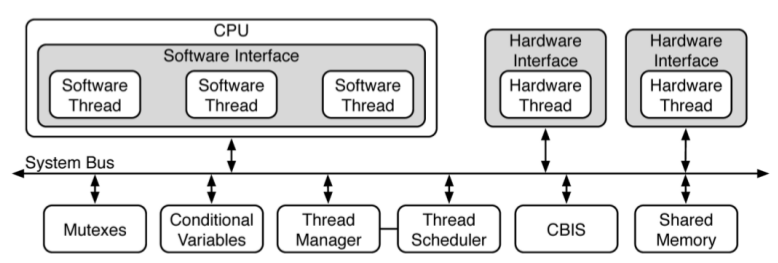
\includegraphics[width=12cm]{../figures/hthreads}
	\caption{Hthreads system block diagram \citep{ASA08}}
	\label{fig:hthreads}
\end{figure}
Instead of utilizing an existing \ac{OS} and its functions through a delegate
mechanism, it implements all resources together with scheduling and management
components in the reconfigurable fabric \citep{ASA08}. While this guarantees a
low-latency access to all components, the central system bus limits the
overall performance in high-load situation and the architecture is rather
unportable to standard \ac{OS} kernels or other platforms. However,
implementing  \ac{OS} functions on the \ac{FPGA}, seems to be the best
approach to utilize the full potential of a parallel hardware design in a
hybrid multi-core system. Adopting this idea for the ReconOS framework
promises significant speedups for many applications and seems to be crucial to
utilize ReconOS in modern \ac{PAC} designs.

Besides the implementation of \ac{OS} functions in hardware, both software and
hardware threads must be able to access these functions transparently through
a central interconnect. While hthreads utilizes a central bus for this task, a
bus structure, again, limits parallel access and performance. Choosing an
appropriate interconnect, just like the implementation mode of the resources,
seems to be a crucial step, highly dependent on the application and its
structure. Furthermore, since the system might be able to adapt itself to
upcoming requirements during runtime, the needs for the interconnect structure
might change after design time. Consequently, an interconnect architecture
should provide a flexible way of utilizing different structures specified at
design time and, additionally, allow a reconfiguration at runtime.

Figure \ref{fig:interconnect} illustrates the reconfigurable interconnect
architecture developed and presented in this thesis.
\begin{figure}
	\centering
	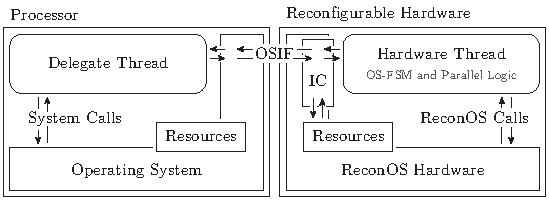
\includegraphics[width=12cm]{../figures/interconnect}
	\caption{Reconfigurable interconnect}
	\label{fig:interconnect}
\end{figure}
It seamlessly integrates into the existing ReconOS architecture by utilizing
the existing interfaces. Instead of connecting the \ac{FIFO} based \acp{OSIF}
directly to the processor, the interconnect allows requests to be rerouted to
resources implemented on the \ac{FPGA}, by introducing a simple addressing
scheme together with a protocol described later. The hardware resources are
also connected to the interconnect via a \ac{FIFO} based interface and
communicate via messages to the different threads. To provide transparent
access to them, the idea of a delegate thread is adopted for software threads,
allowing them to interface with the system the same way a hardware threads
does. While the interconnect presents a fixed interface to the outside world,
its internal structure is hidden completely. This allows to implement
different structures, for example buses, rings, or crossbar interconnects, and
also allows internal reconfiguration at runtime without effecting the
connected components.

The following subsections describe the interconnect in detail and illustrate
its principles. Starting with an introduction of the extended \ac{OSIF}
protocol and its consequences for the software implementation, the software
delegate mechanism is explained and to what extend it allows transparent
access to the hardware resources. Finally, the integration into the existing
ReconOS toolchain will be considered.

\subsection{Interconnect Protocol}
The interconnect routes \ac{OSIF} messages between the different components,
mainly resources, hardware-, software-, and delegate threads. While the
original \ac{OSIF} was intended to be a point-to-point connection between the
hardware and its associated delegate thread, an addressing scheme was not
necessary and, additionally, the length of messages were defined implicitly by
its commands. For an interconnect routing messages to different destinations,
a more advanced protocol is required. Besides, at least, a destination
address, the interconnect also requires knowledge of the length of a message.
Figure \ref{fig:proto} shows the structure of a control word introduced for
the interconnect and send before the start of a message. To minimize the
changes of the hardware thread interface, they are not indicated by a separate
control flag.
\begin{figure}
	\centering
	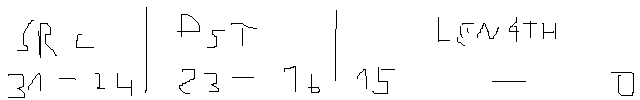
\includegraphics[width=12cm]{../figures/proto}
	\caption{Control message preceding each message}
	\label{fig:proto}
\end{figure}
They consists out of a source and destination, as well as a length field,
indicating the number of following words. Since the address fields have a
length of eight bits, the number of addressable components is limited to 255,
which seems to be sufficient for typical applications. Anyway, the number of
threads and resources is limited by the available resources on the
\ac{FPGA}, as well as routing restrictions. The 16 bit wide length field
allows messages with a maximum number of 65,535 words, which, again, seems to
be sufficient for typical applications. However, it does not allow an endless
streaming of data, which must be split up into messages of fixed size.

For the hardware thread interface, the addressing scheme implies only marginal
changes. The \ac{OSIF} protocol itself remains unchanged, but is preceded by
the additional control word. However, it should be stated, how the control
world is composed for the different \ac{OSIF} calls. The length of a request
is set according to the command and, thereby, known implicitly. Although a
regular request should be routed to the delegate thread, the request itself
must be addressed to the targeted resource. This allows to transparently route
the request not to the delegate thread, but to a resource implemented in
hardware. Addressing such a request with the address of a delegate thread
would prevent such a transparent rerouting. To send back an acknowledge or
response to the hardware thread's request, the receiver must know the source
address, the request is originating from. Therefore, a hardware thread needs
to specify its own id as the source of the request. However, a thread does not
know its own id implicitly, since it depends on the execution mode and
scheduled slot determined at runtime. Consequently, an appropriate mechanism
is needed, allowing a thread to receive its runtime id. Querying the id
through a traditional \ac{OSIF} command is not possible, since the request
itself would require an id. Therefore, the ReconOS runtime sends, initially on
thread creation, the runtime id to the thread, which is responsible for storing it.

Introducing an addressing scheme for the different threads allows to simplify
the interface to the processor. Originally, each of the \acp{OSIF} were
attached individually through a set of memory mapped registers to the
processor. However, since the kernel driver and system bus supports only
sequential access, the parallel mapping could not be utilized for parallel
access and provides no performance benefits. Therefore, the interconnect
provides only a single \ac{FIFO} interface to the processor and is responsible
to arbitrate the different requests from the hardware components. In software,
the driver module provides an interface to wait for and receive messages based
on a filter, specifying a mask (\lstinline{MASK}) and a reference value
\lstinline{BITS}. Whenever the driver module reads a message, it routes it to
the appropriate user-space process satisfying \lstinline{CTRL & MASK == BITS}.
To specify the filter, a process issues the \lstinline{RECONOS_OSIF_SET_MASK}
and \lstinline{RECONOS_OSIF_SET_BITS} system-calls after opening the
appropriate device file. For example, a delegate thread associated to slot 1
needs to receive all messages originating from the associated hardware thread
and specifies a mask of \lstinline{0xFF000000}, together with a reference
value of \lstinline{0x01000000}. It only filters the source address, since the
destination address does not represent the delegate thread, but a specific
resource.

\subsection{Software Delegate Mechanism}

\subsection{Toolchain Integration}

\section{Implementation}
\section{Evaluation}
\begin{itemize}
\item measure time differences for old/new
\item show speedup/speeddown
\end{itemize}